% !TEX TS-program = pdflatex
% !TEX encoding = UTF-8 Unicode
% !TEX ROOT = main.tex

\section{Internet \& Strom}
  % Bild einer Schweinenase <- dies ist keine Steckdose
\paragraph{WLAN}
Das Internet \dots Jeder braucht es und bei uns gibt's das. Praktischerweise habt ihr an den meisten Ecken und erst Recht an unserer Uni öffentliches WLAN. Wenn ihr schon im Netz ``eduroam'' registriert seid, weil es das an eurer Hochschule auch gibt - super! Ihr könnt euch zurücklehnen und braucht gar nichts weiter zu machen.

Wenn ihr noch nicht direkt verbunden werdet oder schlichtweg keinen Zugang habt, gibt es hier auch das öffentliche Netz ``Heidelberg4You''. Es ist überall dort verfügbar, wo die ZaPFika neben euch im ``eduroam'' sind und sogar noch an weiteren Stellen in Heidelberg. Die Anmeldung dort funktioniert recht einfach über ein Pop-Up Window, in dem ihr einfach die Lizenzbedingungen \textit{lesen} und bestätigen müsst. Danach habt ihr unbegrenzten Internetzugang, um noch produktiver für die ZaPF zu arbeiten oder euch von der NSA abhören zu lassen. Um letzteres zu verhindern, bietet sich auch die Verwendung eines Virtuel Private Network (VPN) an.

\paragraph{Drucken}
Solltet ihr mal lebenswichtige Papiere auszudrucken haben, geht das im Tagungsbüro. Dort gibt es jede Menge Computer, die eure Dateien öffnen können sollten und sich auch mit den Druckern dort verbinden können. Natürlich ist das ganze nicht dazu gedacht, eure ganzen Fotos vom letzten Urlaub auszudrucken (die Qualität ist eh nicht die beste), sondern lediglich dazu, die Resolutionen in Papierform zu haben, den AK Leitern das nötige Material zu beschaffen und solche Tagungsdinge eben, die anfallen.

\paragraph{Strom}
Ein Leben ohne Strom? Undenkbar! Auf den Zimmern der Jugendherbege wird es genug Steckdosen geben, um eure klugen Handys über Nacht zu laden und allen möglichen anderen Shice damit zu machen. In den AK Räumen gibt es auf der Fensterseite genug Steckdosen, wenn eurem Laptop doch tagsüber auch mal der Saft ausgeht. In dem Plenums Hörsaal wird ebenfalls für ausreichend Anschlüsse gesorgt, damit es währenddessen auch schön spannend bleibt. Da der ein oder andere von euch aus Versehen die Verlängerungskabel vergessen haben wird, liegen auch ein paar im Tagungsbüro aus. Und wenn es wie im nächsten Bild aussieht, habt ihr schon viel richtig gemacht.
\todo[inline]{Kabel Rätsel als svg (mit includesvg)}
\begin{figure}[h]
\centering
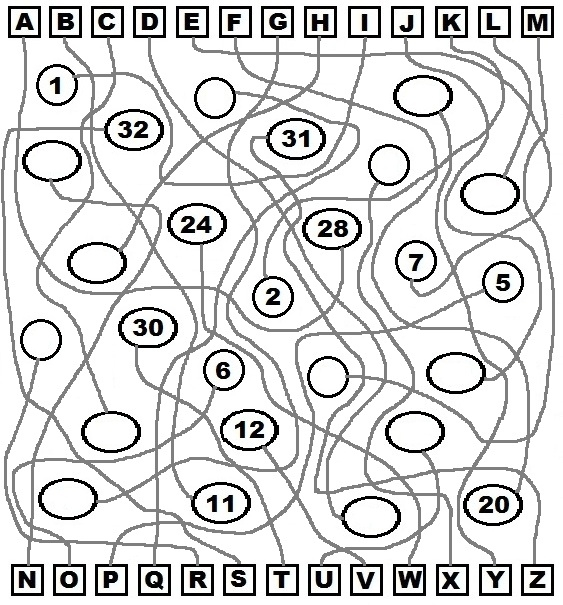
\includegraphics[width=\textwidth]{chapters/survive/kabel_raetsel.jpg}
\end{figure}
Übrigens: Stecker passen beidseitig ;)
\todo[inline]{passende Fotos raussuchen}
